\cleardoublepage

\chapter{Sigfox}

\begin{wrapfigure}{r}{3cm}
\Youtube{https://youtu.be/mLZoeHE5Gaw}
\end{wrapfigure}


\lgf{\Index{Sigfox} est l'un des tous premiers réseaux entièrement dédié à l'Internet des Objets. Comme nous l'avons vu auparavant, il est de la famille des \Index{LPWAN} qui privilégie la portée et la consommation d'énergie au débit. Les communications sont également fortement asymétrique, ce qui fait que les échanges ne sont pas comme sur un réseau Wi-Fi. }
\lge{\Index{Sigfox} is one of the very first networks entirely dedicated to the Internet of Things. As we have seen before, it belongs to the \Index{LPWAN} family, which favors range and energy consumption over throughput. The communications are also highly asymmetrical, which means that the exchanges are not like on a Wi-Fi network. }


     \vspace{1em}

\lgf{Les LoPy peuvent utiliser le réseau et bénéficie d'un an de connectivité gratuite sur le réseau Sigfox. Après les coûts d'abonnement sont relativement limités.}
\lge{LoPy can use the network and benefits from one year of free connectivity on the Sigfox network. After that the subscription costs are relatively limited.}


\lgf{\section{Récupération des identifiants}}
\lge{\section{Retrieving identifiers}}

\lgf{Dans un premier temps, vous devez enregistrez votre capteur sur le site de Sigfox. Il vous faut deux éléments : son identifiant et son mot de passe appelé \ac{PAC}. Ce dernier doit rester secret car il permet à toute personne qui le possède d’enregistrer un objet ou d’en changer le propriétaire.}
\lge{First, you must register your sensor on the Sigfox website. You need two elements: its identifier and its password called \ac{PAC}. The latter must remain secret because it allows anyone who has it to register an object or change its owner.}


\lgf{Le programme \lprog{sigfox\_id.py}{pycom} permet d’afficher ces deux valeurs et d’envoyer un message sur le réseau Sigfox. 
Avant de l’exécuter, vérifiez que vous avez branché une antenne sur le connecteur de droite, celui opposé au bouton Reset sur le Pycom, coté LED.}
\lge{The program \lprog{sigfox\_id.py}{pycom} allows to display these two values and to send a message on the Sigfox network. 
Before running it, check that you have connected an antenna on the right connector, the one opposite to the Reset button on the Pycom, LED side.}


\pycomlst{sigfox\_id.py} 

\lgf{Ce programme importe l’objet \pfunction{network}{Sigfox} du module \texttt{network} (ligne 1) et crée une instance \texttt{sigfox} (ligne 10). Il est important de bien spécifier la bonne région d’utilisation car les bandes de fréquences peuvent différer d'un continent à un autre. En plus d’émettre dans l’illégalité, le réseau Sigfox ne recevra pas les messages.}
\lge{This program imports the \pfunction{network}{Sigfox} object from the \texttt{network} module (line 1) and creates an instance of \texttt{sigfox} (line 10). It is important to specify the right region of use because frequency bands can differ from one continent to another. In addition to transmitting illegally, the Sigfox network will not receive the messages.}

\lgf{Les lignes 13 et 16 affichent les identifiants Sigfox de votre LoPy. Notez-les, ils nous serviront pour enregistrer l’objet sur le réseau de Sigfox.}
\lge{Lines 13 and 16 display the Sigfox identifiers of your LoPy. Note them, they will be used to register the object on the Sigfox network.}

\lgf{La ligne 18 crée une \pfunction{socket}{socket}, à l’instar de ce qui avait été fait avec UDP au chapitre précédent. On peut donc utiliser les mêmes primitives en Sigfox qu’en UDP. La ligne 19 permet d’envoyer un message que vous pouvez personnaliser dans la limite de 12 caractères~; taille maximale des trames Sigfox.}
\lge{Line 18 creates a function{socket}{socket}, like what was done with UDP in the previous chapter. So we can use the same primitives in Sigfox as in UDP. The line 19 allows to send a message that you can customize within the limit of 12 characters~; maximum size of Sigfox frames.}

\lgf{\section{Enregistrement de l'objet}}
\lge{\section{Object registration}}

\lgf{Maintenant que vous avez les précieux identifiants Sigfox, connectez-vous avec un navigateur sur le site \url{https://backend.sigfox.com/activate}. Le processus est très simple. Il suffit de remplir les champs des différents formulaires~:}
\lge{Now that you have the precious Sigfox identifiers, connect with a browser to the site \url{https://backend.sigfox.com/activate}. The process is very simple. You just have to fill the fields of the different forms:}

\begin{itemize}
    \item 
        \lgf{indiquez votre pays ;}
        \lge{indicate your country;}
    \item  
        \lgf{remplissez le formulaire avec l'identifiant de l'objet et le \Index{PAC} que vous avez obtenus avec le programme \lprog{sigfox\_id.py}{pycom} ;}
        \lge{fill in the form with the object identifier and the \Index{PAC} that you obtained with the program \lprog{sigfox\_id.py}{pycom} ;}
    \item  
        \lgf{indiquez à des fins de statistique ce qui vous amène ici ;}
        \lge{indicate for statistical purposes what brings you here;}
    \item  
        \lgf{créez votre compte Sigfox.}
        \lge{create your Sigfox account.}
\end{itemize}

\lgf{Ce qui va conduire à enregistrer l’objet et à vous créer un compte sur le backend de Sigfox.}
\lge{This will lead to register the object and create an account on the Sigfox backend.}


\lgf{\section{Visualisation des données émises par le Pycom}}
\lge{\section{Visualization of the data issued by the Pycom}}


\lgf{Rendez-vous sur le \Index{backend} de Sigfox (\url{https://backend.sigfox.com/}) et identifiez-vous avec le compte que vous venez de créer.}
\lge{Go to the Sigfox website (\url{https://backend.sigfox.com/}) and identify yourself with the account you just created.}

\begin{figure}[tbp]
\centerline{
\includegraphics[width=1\columnwidth]{Pictures/sigfox-accueil.png} }
\lgf{\caption{Page d'accueil}}
\lge{\caption{Home page}}
\label{fig-sigfox-accueil}
\end{figure}

\lgf{Les onglets en haut de la page (cf. figure~\vref{fig-sigfox-accueil}) vont vous permettre de naviguer dans différents types d’information. Dans cette partie, nous n'utiliserons que l'onglet \textit{DEVICE}. Il donne accès aux objets enregistrés vous appartenant (cf.figure~\vref{fig-sigfox-device}). On y retrouve~:}
\lge{The tabs at the top of the page (see figure~vref{fig-sigfox-home}) will allow you to navigate through different types of information. In this part, we will only use the tab \textit{DEVICE}. It gives access to the registered objects belonging to you (see figure~\vref{fig-sigfox-device}). It contains:}

\begin{figure}[tbp]
\centerline{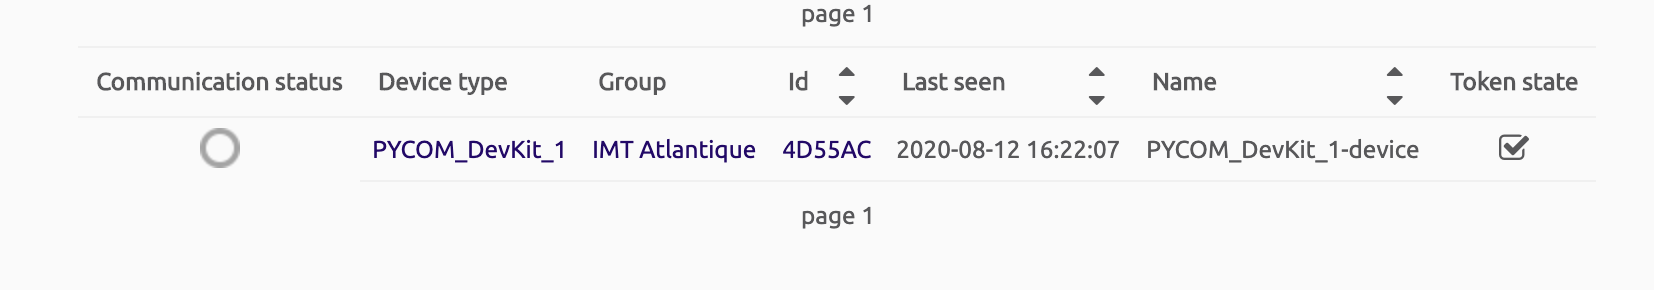
\includegraphics[width=1\columnwidth]{Pictures/sigfox-device.png} }
\lgf{\caption{Objets enregistrés}}
\lge{\caption{Registered objects}}
\label{fig-sigfox-device}
\end{figure}

\begin{itemize}
    \item 
        \lgf{un nom créé par Sigfox en fonction du type d’objet~; }
        \lge{a name created by Sigfox according to the type of object; }
    \item  
        \lgf{le propriétaire~;}
        \lge{the owner;}
    \item  
        \lgf{l’ID que vous avez donnés lors de l’enregistrement~;}
        \lge{the ID you gave when you registered;}
    \item  
        \lgf{la date du dernier message reçu par Sigfox pour cet objet.}
        \lge{the date of the last message received by Sigfox for this object.}
\end{itemize}

     \vspace{1em}

\lgf{Il faut cliquer~:}
\lge{You must click:}
\begin{itemize}
    \item 
        \lgf{sur le nom de l’objet pour le configurer~;}
        \lge{on the object name to configure it;}
    \item 
        \lgf{sur le nom du groupe pour accéder à des paramètres d’administration des objets~;}
        \lge{on the group name to access object administration settings;}
    \item 
        \lgf{sur l’ID de l’objet pour obtenir des informations concernant les messages reçus puis \textit{MESSAGES} dans le menu de gauche, pour avoir la liste des messages reçus par Sigfox, comme montré à la figure~\vref{fig-sigfox-message}\footnote{La séquence \texttt{48 69 21 20 53 69 67 66 6f 78} correspondant à la chaîne de caractères \texttt{Hi! Sigfox}.}.}
        \lge{on the object ID to get information about the received messages then \textit{MESSAGES} in the left menu, to get the list of messages received by Sigfox, as shown in figure~\vref{fig-sigfox-message}\footnote{The sequence \texttt{48 69 21 20 53 69 67 66 6f 78} corresponding to the string \texttt{Hi! Sigfox}.}}
\end{itemize}



\begin{figure}[tbp]
\centerline{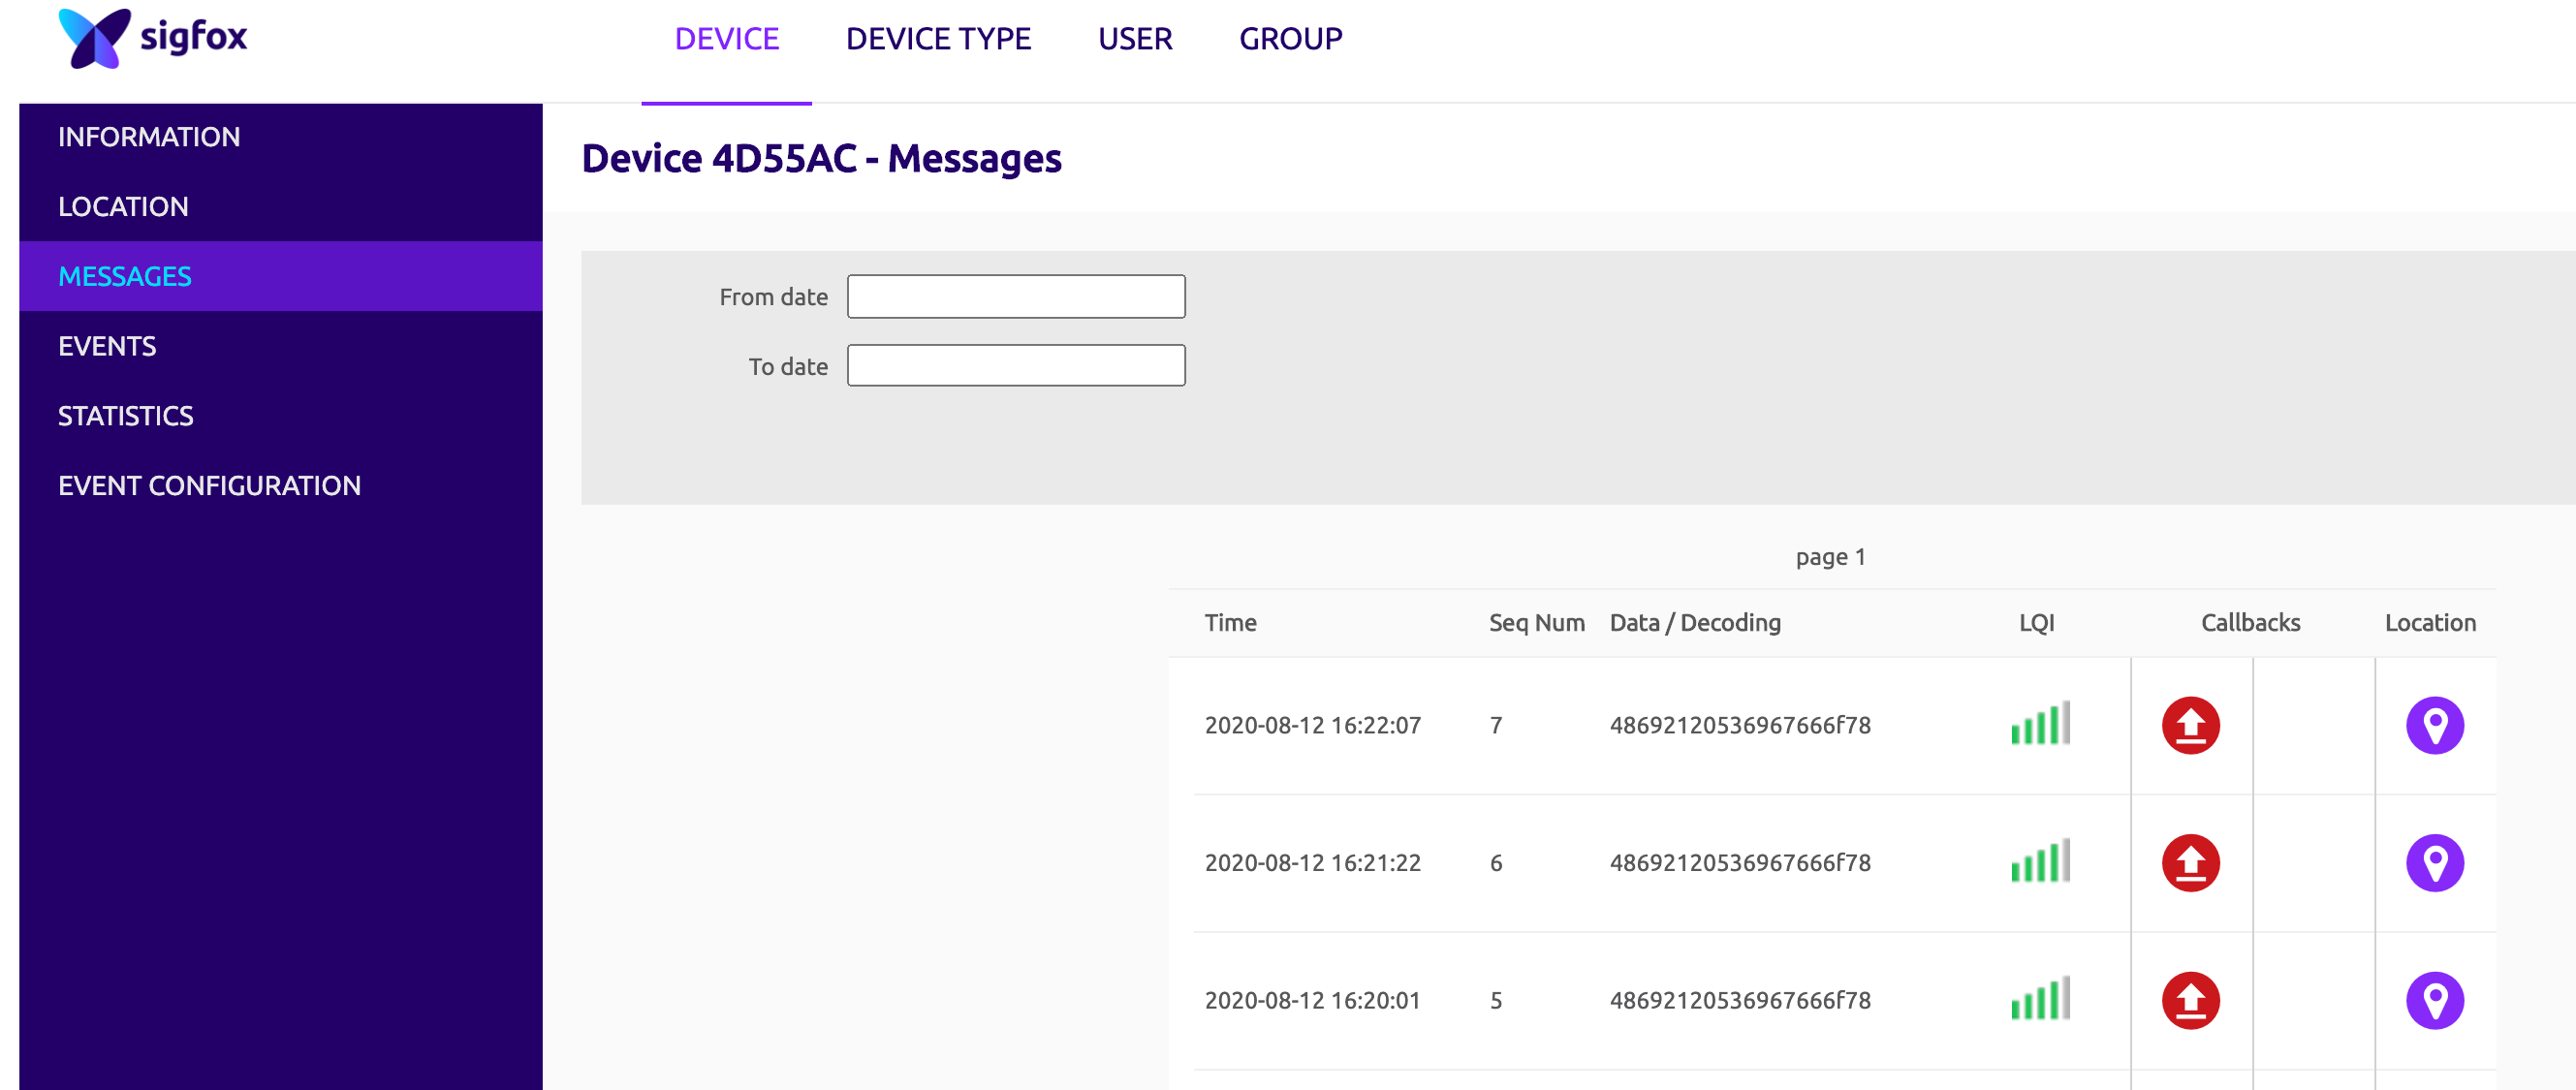
\includegraphics[width=1\columnwidth]{Pictures/sigfox-message.png} }
\lgf{\caption{Liste des messages reçus}}
\lge{\caption{List of received messages}}
\label{fig-sigfox-message}
\end{figure}

\lgf{\section{Que s'est-il passé coté radio}}
\lge{\section{What happened on the radio side}}

\lgf{La figure~\vref{fig-sigfox-spectrum} montre sur un \Index{analyseur de spectre}, l'émission de 4 trames de données, dont une en cours, par un objet. Les petits traits verticaux correspondent à une émission. Ces traits sont très fin ; la bande passante utilisée est très petite, d'où le terme anglais de \ac{UNB}. Cela limite le risque de \Index{collision} qui rendrait la donnée incompréhensible lié à l'émission simultanée d'un autre équipement sur la même fréquence. }
\lge{The figure~\vref{fig-sigfox-spectrum} shows on a \Index{spectrum analyzer}, the emission of 4 frames of data, including one in progress, by an object. The small vertical lines correspond to an emission. These lines are very fine; the bandwidth used is very small, hence the term \ac{UNB}. This limits the risk of \Index{collision} which would make the data incomprehensible linked to the simultaneous emission of another equipment on the same frequency. }

\lgf{En fait, le même message est émis 3 fois sur des fréquences différentes et aléatoire, augmentant ses chances d'être reçu. }
\lge{In fact, the same message is transmitted 3 times on different and random frequencies, increasing its chances of being received. }

\begin{figure}[tbp]
\centerline{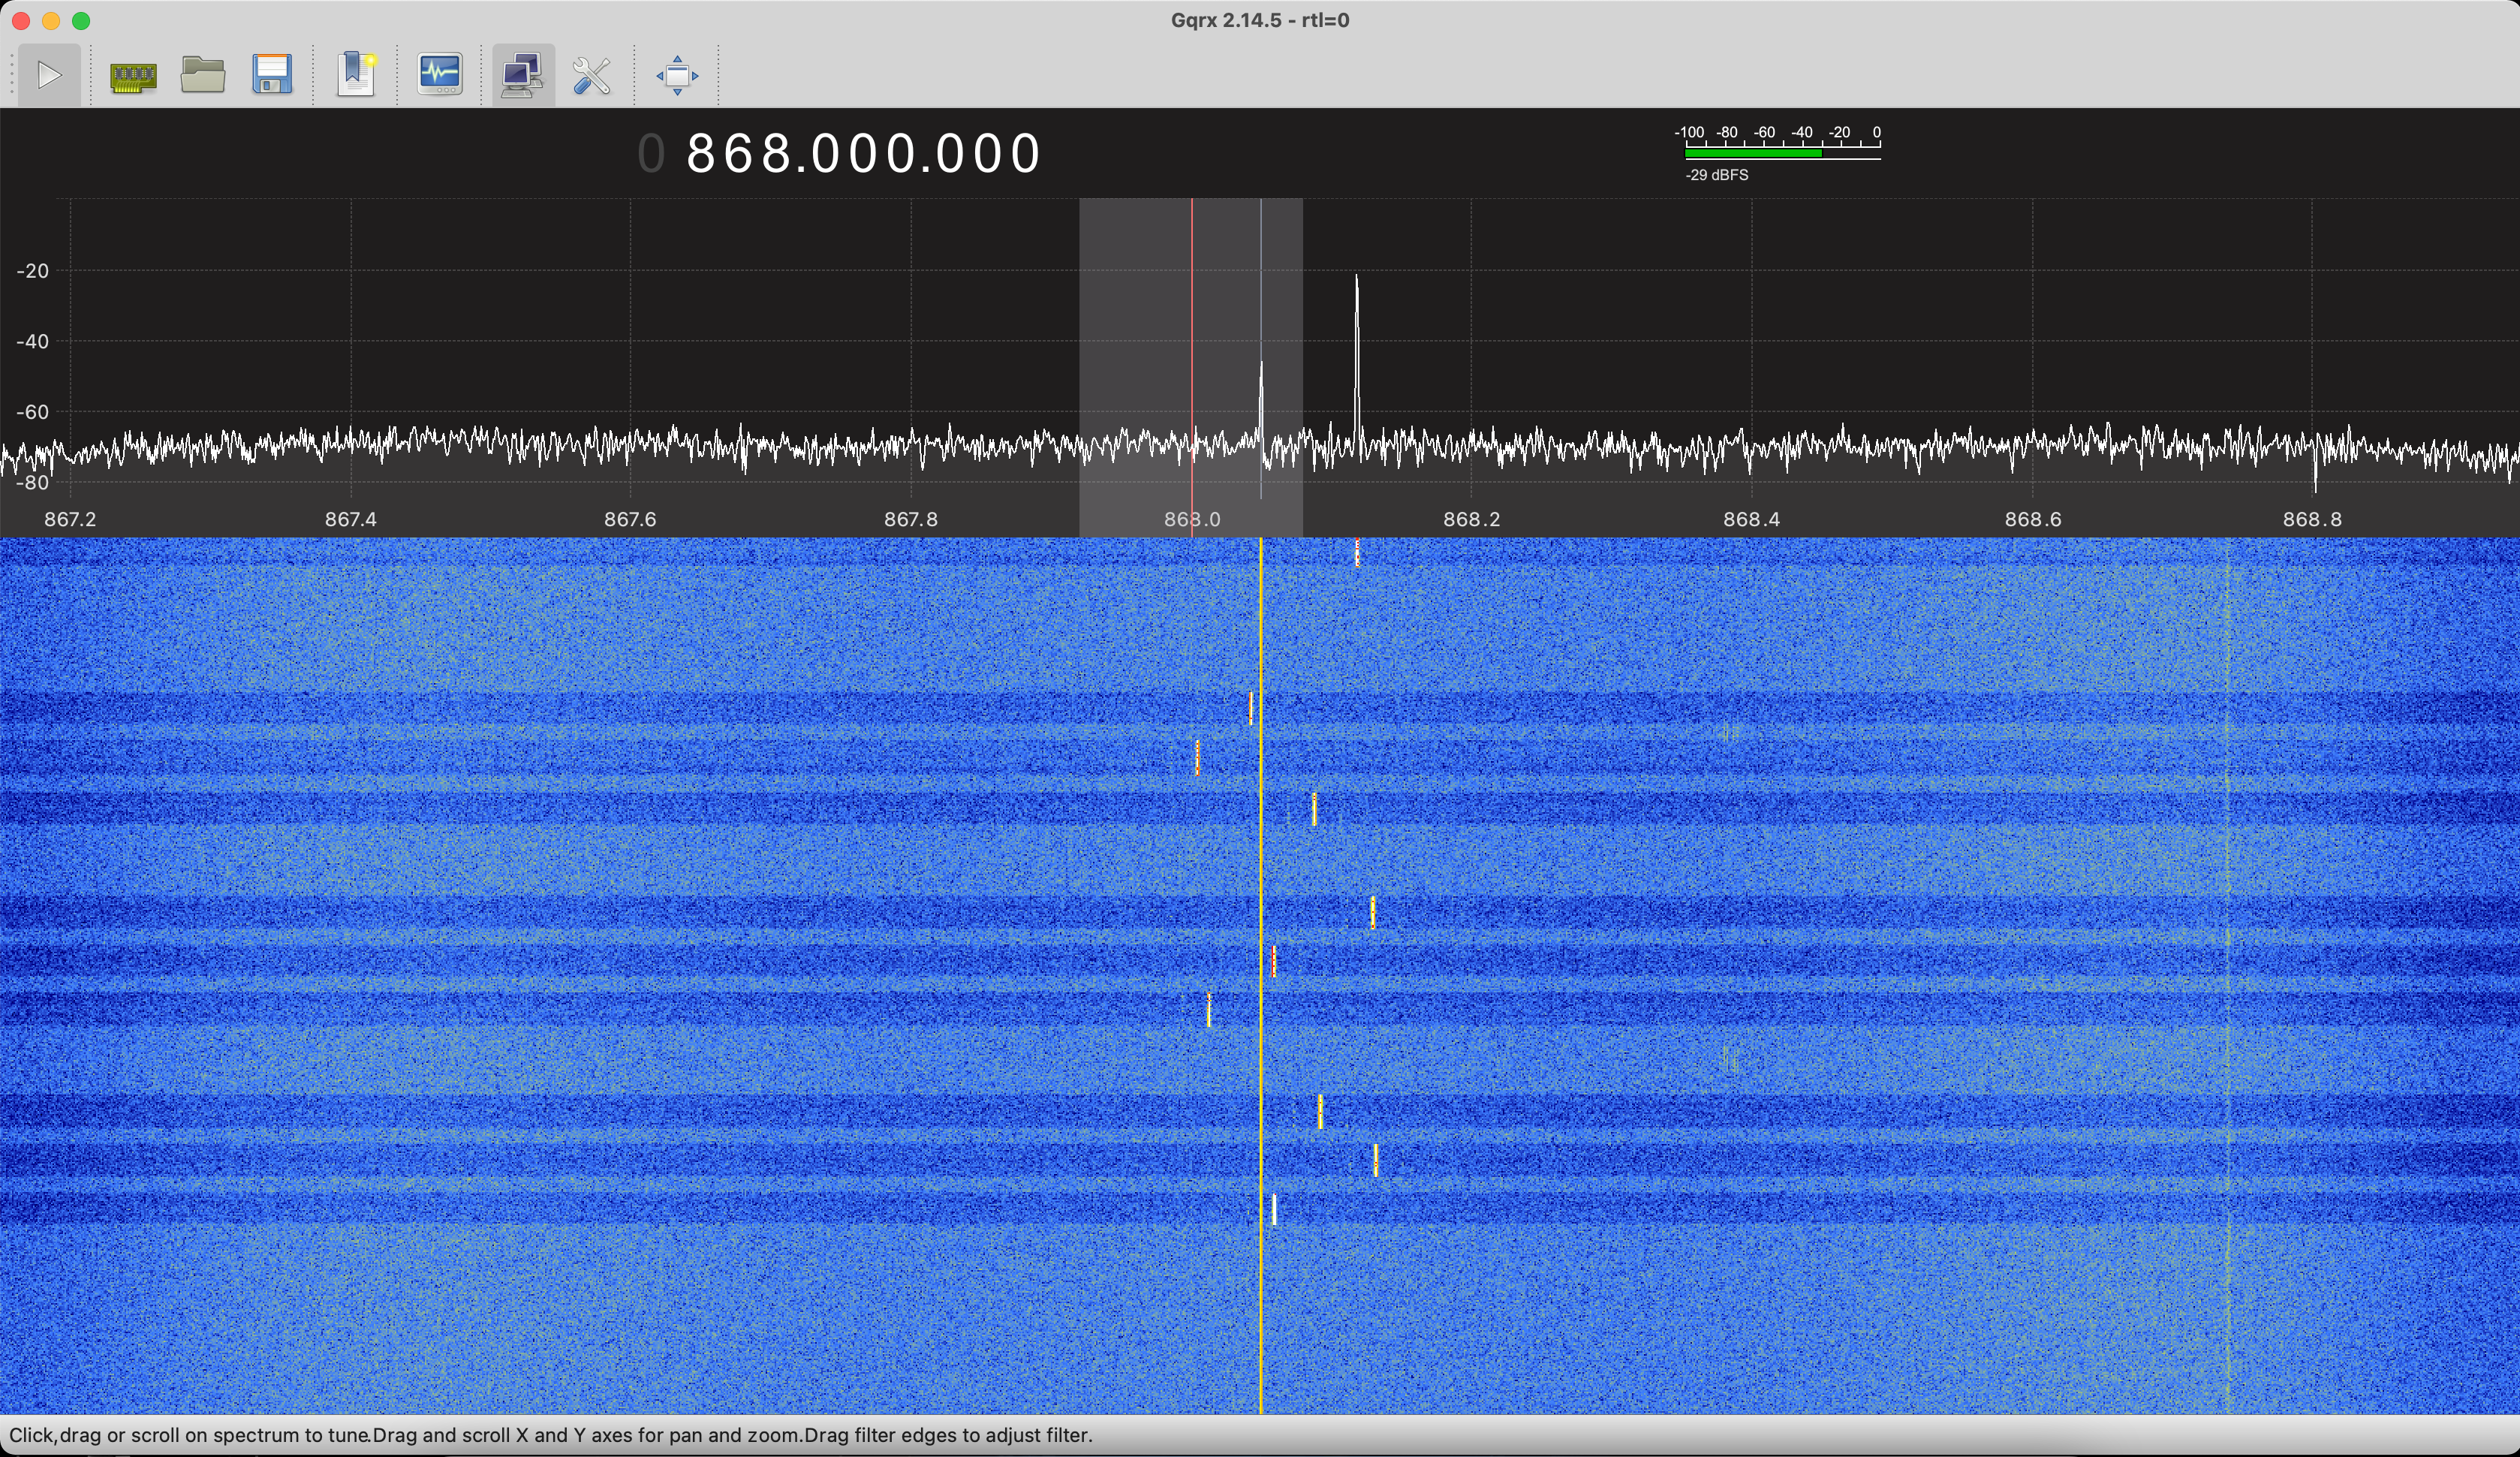
\includegraphics[width=1\columnwidth]{Pictures/sigfox-spectrum.png} }
\lgf{\caption{Émissions radio liées à l'envoi de trame Sigfox.}}
\lge{\caption{Radio emissions related to the sending of Sigfox frames.}}
\label{fig-sigfox-spectrum}
\end{figure}

\lgf{\section{Récupération des données}}
\lge{\section{Data retrieval}}

\begin{wrapfigure}{r}{3cm}
\Youtube{https://youtu.be/wBccbspakV0}
\end{wrapfigure}

\lgf{L'idéal serait d’avoir directement accès à ces données pour pouvoir les manipuler dans un programme. Pour ce faire, nous pouvons utiliser l’API REST développée par Sigfox.
Dans l’onglet \textit{DEVICE} (figure~\vref{fig-sigfox-device}), il faut cliquer cette fois ci sur~:}
\lge{Ideally, we would like to have direct access to this data in order to manipulate it in a program. To do this, we can use the REST API developed by Sigfox. In the tab \textit{DEVICE} (figure~\vref{fig-sigfox-device}), we have to click this time on:}

\begin{itemize}
    \item 
        \lgf{le nom de votre groupe~;}
        \lge{the name of your group;}
    \item  
        \lgf{dans le menu de gauche, sur \texit{API ACCESS}~;}
        \lge{from the left-hand menu, select \texit{API ACCESS};}
    \item  
        \lgf{en haut à droite, sur le tout petit bouton \textit{New}.}
        \lge{at the top right, on the very small button \textit{New}.}
\end{itemize}

\lgf{Une page similaire à la figure~\vref{fig-sigfox-api} s'affiche. Donnez un nom à cet accès et choisissez, dans le menu \textit{Profiles} le choix \textit{DEVICE MESSAGE [R]} pour avoir le droit de lire les messages. Puis évidemment, sur \texit{Ok}.}
\lge{A page similar to figure~ref{fig-sigfox-api} is displayed. Give a name to this access and choose, in the menu \textit{Profiles} the choice \textit{DEVICE MESSAGE [R]} to have the right to read the messages. Then, of course, click on \texit{Ok}.}


     \vspace{1em}

\lgf{Vous voyez apparaître une nouvelle page avec deux champs en hexadécimal~: \textit{login} et \textit{password}, que vous devez, comme pour l'API de Beebotte, noter quelqe part ou apprendre par cœur pour la suite.}
\lge{You see a new page with two fields in hexadecimal: \textit{login} and \textit{password}, that you must, as for the Beebotte API, write down somewhere or learn by heart for the following.}

\lgf{Le mieux étant de remplir un fichier de configuration avec ces valeurs comme le montre le programme \lprog{config\_sigfox.py}{pycom}.}
\lge{The best is to fill a configuration file with these values as shown in the program \lprog{config\_sigfox.py}{pycom}.}


\pycomlst{config\_sigfox.py}


\begin{figure}[tbp]
\centerline{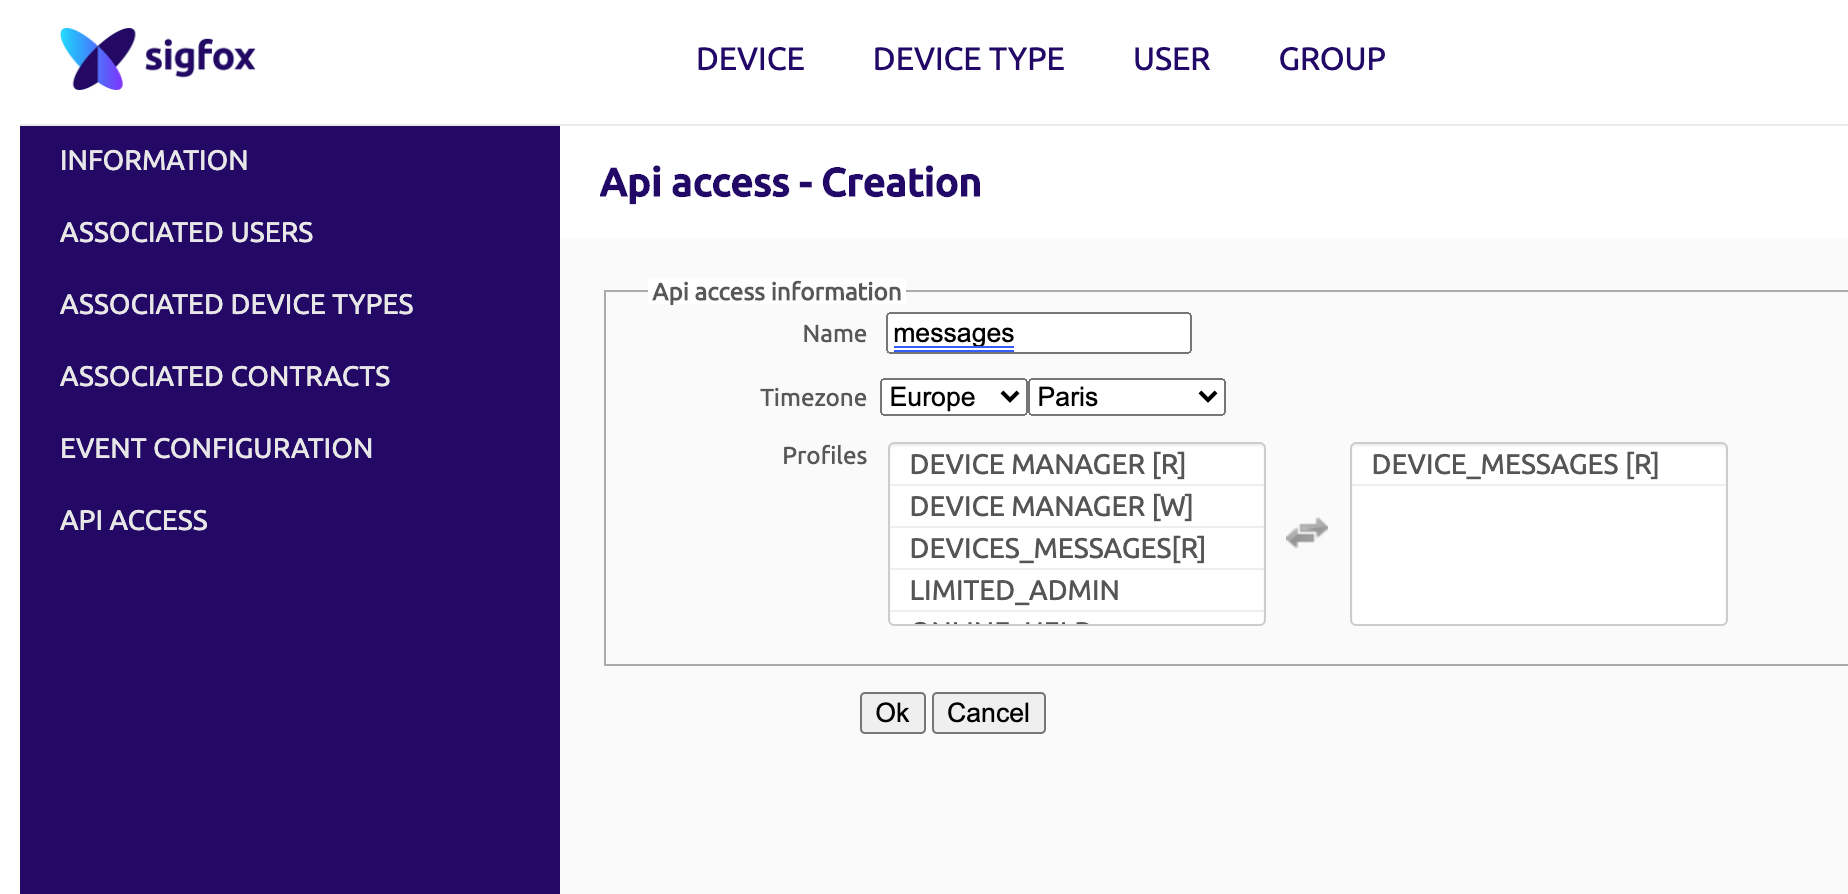
\includegraphics[width=1\columnwidth]{Pictures/sigfox-api-access.png} }
\lgf{\caption{Configuration de l'API REST.}}
\lge{\caption{REST API configuration.}}
\label{fig-sigfox-api}
\end{figure}

     \vspace{1em}

\lgf{Tous les éléments sont maintenant réunis pour émettre un relevé de température en utilisant le réseau Sigfox. }
\lge{All the elements are now in place to transmit a temperature reading using the Sigfox network. }

\subsection{Sur le serveur}

\lgf{Nous avons les clés d’accès à l’API, il suffit maintenant d’écrire un petit script Python.}
\lge{We have the access keys to the API, now we just need to write a small Python script.}

\lgf{Pour des raisons de sécurité, nous vous invitons à prendre l'habitude de mettre les informations sensibles dans un fichier séparé.}
\lge{For security reasons, we invite you to make a habit of putting sensitive information in a separate file.}

\lgf{Le programme \pprog{device\_messages.py}{plido-tp3} permet de lister les messages reçus par Sigfox pour un objet particulier sur votre ordinateur.}
\lge{The program \pprog{device\_messages.py}{plido-tp3} allows to list the messages received by Sigfox for a particular object on your computer.}


\pythonlst{device\_messages.py}

Le programme~:
\begin{itemize}
    \item 
        \lgf{Ligne 1, importe le module \texttt{requests} pour pouvoir envoyer des requêtes http à un serveur.}
        \lge{Line 1, import the module \texttt{requests} to be able to send http requests to a server.}
    \item  
        \lgf{Ligne 3, le module \pfunction{requests}{HTTPBasicAuth} est utilisé pour s'identifier de façon simple en utilisant un login et un mode de passe.}
        \lge{Line 3, the module \pfunction{requests}{HTTPBasicAuth} is used to identify itself in a simple way using a login and a password.}
    \item  
        \lgf{Ligne 6 ce login et ce mot de passe sont extrait du fichier rempli au chapitre précédent lors de la création de l'API REST.}
        \lge{Line 6 this login and password are extracted from the file filled in the previous chapter when the REST API was created.}
    \item  
        \lgf{Ligne 9, l’URL comportant l’ID de l'objet est construite et }
        \lge{Line 9, the URL with the object ID is built and }
    \item  
        \lgf{ligne 13 la requête HTTP est envoyée avec la méthode d’authentification basée sur le mot de passe. la variable  \texttt{r} est une structure contenant plusieurs informations. }
        \lge{line 13 the HTTP request is sent with the authentication method based on the password. the variable \texttt{r} is a structure containing several information. }
    \item  
        \lgf{Lignes 14 à 17, Si le code retourné est 200, tout s’est bien passé et \texttt{r.text} contient la réponse.}
        \lge{Lines 14 to 17, If the returned code is 200, everything went well and \texttt{r.text} contains the answer.}
    \item  
        \lgf{Ligne 19, cette réponse est une chaîne de caractères qui est désérialisée de la représentation JSON pour en faire une structure Python grâce à la fonction \pfunction{json}{loads}.}
        \lgf{Line 19, this response is a string that is deserialized from the JSON representation to a Python structure using the function \pfunction{json}{loads}.}
    \item  
        \lgf{Ligne 20, la réponse est affichée et ensuite certains éléments sont donnés. On y retrouve tous les messages qui ont été émis par le LoPy.}
        \lge{Line 20, the answer is displayed and then some elements are given. All the messages that have been sent by the LoPy are shown.}
    \end{itemize}


\begin{termc}[backgroundcolor=\color{palerod}, basicstyle=\ttfamily\small, escapechar=@]
>@\textbf{python3 device\_messages.py}@
https://backend.sigfox.com/api/v2/devices/1B28CF4/messages
200
{'data': [{'country': 'FRA',
           'data': '48692120536967666f78',
           'device': {'id': '1B28CF4'},
           'lqi': 3,
           'nbFrames': 3,
           'operator': 'SIGFOX_France',
           'rinfos': [],
           'rolloverCounter': 0,
           'satInfos': [],
           'seqNumber': 13,
           'time': 1640279367000},
          {'country': 'FRA',
           'data': '48692120536967666f78',
  ...
           'rolloverCounter': 0,
           'satInfos': [],
           'seqNumber': 11,
           'time': 1640279155000}],
 'paging': {}}
1640279367000: 13 48692120536967666f78  [b'Hi! Sigfox']  received 0
1640279338000: 12 48692120536967666f78  [b'Hi! Sigfox']  received 0
1640279155000: 11 48692120536967666f78   [b'Hi! Sigfox']  received 0
\end{termc}

\lgf{La fin de la trace affiche un résumé plus lisble de l'information reçue~:}
\lge{The end of the trace displays a more readable summary of the information received:}

\begin{itemize}
    \item  
        \lgf{\texttt{time} donne l’heure de réception codée suivant le format \Index{Epoch}, évoqué lors de la communication avec Beebotte au chapitre précédent~;}
        \lge{\texttt{time} gives the reception time coded according to the format \Index{Epoch}, mentioned during the communication with Beebotte in the previous chapter~;}
    \item  
        \lgf{\texttt{seqNumber} contient le numéro de la trame et est remis a 0 quand l’objet est reflashé. Il permet de détecter des pertes de données si les numéros ne sont pas contigu~; }
        \lge{\texttt{seqNumber} contains the frame number and is reset to 0 when the object is reflashed. It allows to detect data loss if the numbers are not contiguous; }
    \item  
        \lgf{"data" contient les données codées dans une chaîne hexadécimale. Le programme utilise la fonction \pfunction{binascii}{unhexifily} pour la reconvertir en séquence d’octets qui peuvent être affichés s’il s’agit de caractères ACSII~;}
        \lge{"data" contains the data encoded in a hexadecimal string. The program uses the function \pfunction{binascii}{unhexifily} to convert it back into a sequence of bytes that can be displayed if they are ACSII~ characters;}
    \item  
        \lgf{\texttt{rinfos} donne les informations sur les différentes passerelles radio de l’opérateur qui ont reçu le message.}
        \lge{\texttt{rinfos} gives the information about the different radio gateways of the operator that received the message.}
\end{itemize}


\lgf{\subsection{Sur le LoPy}}
\lge{\subsection{On the LoPy}}

\lgf{Le programme \lprog{sigfox\_temperature.py}{pycom} est une adaptation de \lprog{wifi\_temperature.py}{pycom}, listing~\vref{prog-wifi-temp} dédié au Wi-Fi pour des transmission sur le réseau Sigfox.}
\lge{The program \lprog{sigfox\_temperature.py}{pycom} is an adaptation of \lprog{wifi\_temperature.py}{pycom}, listing~\vref{prog-wifi-temp} dedicated to Wi-Fi for transmission on the Sigfox network.}

\pycomlst{sigfox\_temperature.py}

\begin{itemize}
    \item 
        \lgf{ligne 5, la classe \pfunction{network}{Sigfox} du module \texttt{network} est installée~;}
        \lge{line 5, the \pfunction{network}{Sigfox} class of the \texttt{network} module is set up;}
    \item  
        \lgf{ligne 11, un objet \texttt{texttt} est instancié avec, ici, les paramètres pour l'Europe~;}
        \lge{line 11, an object \texttt{texttt} is instantiated with, here, the parameters for Europe;}
    \item  
        \lgf{ligne 12, au lieu de faire appel à \texttt{\Index{AF\_INET}} pour utiliser la pile protocolaire TCP/IP, la valeur \texttt{\Index{AF\_SIGFOX}} est utilisée.}
        \lge{line 12, instead of using \texttt{\Index{AF\_INET}} to use the TCP/IP protocol stack, the value \texttt{\Index{AF\_SIGFOX}} is used.}
    \item  
        \lgf{ligne 14, la taille de la trame est fixée à 12 octets pour être compatible avec le réseau.}
        \lge{line 14, the size of the frame is fixed at 12 bytes to be compatible with the network.}
\end{itemize}

\lgf{Le programme s'exécute sur le LoPy.}
\lge{The program runs on the LoPy.}

\begin{termc}[backgroundcolor=\color{gray!10}, basicstyle=\ttfamily\tiny, escapechar=@]
>>> Running sigfox_temperature.py

>>>
>>>
[118]
[2192] 4
[2192, -89] 6
[2192, -89, -16] 7
[2192, -89, -16, -12] 8
[2192, -89, -16, -12, -15] 9
[2192, -89, -16, -12, -15, -23] 10
[2192, -89, -16, -12, -15, -23, -11] 11
[2192, -89, -16, -12, -15, -23, -11, -14] 12
[2192, -89, -16, -12, -15, -23, -11, -14, -13] 13
[1999, -12] 5
[1999, -12, -5] 6
[1999, -12, -5, -8] 7
[1999, -12, -5, -8, -9] 8
[1999, -12, -5, -8, -9, -6] 9
[1999, -12, -5, -8, -9, -6, 2] 10
[1999, -12, -5, -8, -9, -6, 2, 0] 11
[1999, -12, -5, -8, -9, -6, 2, 0, -5] 12
[1999, -12, -5, -8, -9, -6, 2, 0, -5, -2] 13
[1954, -4] 5
[1954, -4, -1] 6
\end{termc}

\lgf{Le  programme \pprog{device\_messages.py}{plido-tp3} récupère également ces valeurs depuis l'ordinateur.}
\lge{The program \pprog{device\_messages.py}{plido-tp3} also retrieves these values from the computer.}

\begin{termc}[backgroundcolor=\color{palerod}, basicstyle=\ttfamily\tiny, escapechar=@]
1640281923000: 15 891907cf2b24272825020024  [b"\x89\x19\x07\xcf+$'(%\x02\x00$"] received 0
1640281823000: 14 8819089038582f2b2e362a2d  [b'\x88\x19\x08\x908X/+.6*-'] received 0
1640279367000: 13 48692120536967666f78      [b'Hi! Sigfox']      received 0
1640279338000: 12 48692120536967666f78      [b'Hi! Sigfox']      received 0
1640279155000: 11 48692120536967666f78      [b'Hi! Sigfox']      received 0
\end{termc}

\lgf{Attention suivant les variations de la température, le message CBOR grandit plus au moins vite. Dans le cas précédent, il y avait une émission toutes les 90 secondes, or l'abonnement au réseau Sigfox limite le nombre d'émission à 140 messages par jours. Au bout de 3 heures le quota de message sera épuisé. Cette petite période d'émission permet de tester plus rapidement les solutions, mais il convient d'augmenter la période pour une utilisation régulière.}
\lge{Be careful, depending on the temperature variations, the CBOR message grows more or less quickly. In the previous case, there was an emission every 90 seconds, but the subscription to the Sigfox network limits the number of emission to 140 messages per day. At the end of 3 hours the quota of messages will be exhausted. This small period of emission allows to test more quickly the solutions, but it is advisable to increase the period for a regular use.}

\subsection{requête GET depuis le serveur}\label{chap-sigfox-GET}

Côté ordinateur, la stratégie la plus simple à mettre en œuvre consiste à étendre le programme \pprog{device\_message.py}{plido-tp3} vu précédemment et d'interroger périodiquement le \textit{backend} de Sigfox pour voir si de nouvelles données sont arrivées. Cela donne le programme \pprog{display\_sigfox.py}{plido-tp3} suivant~:

\pythonlst[firstline=1,lastline=14, firstnumber=1]{display\_sigfox.py}

Les importations incluent les modules pour envoyer les données à Beebotte et pour interroger Sigfox. Ligne 14, la communication avec les serveur de Beebotte est établie en utilisant les secrets du module \texttt{config\_btt}.

\pythonnxt[firstline=41,lastline=54, firstnumber=41]{display\_sigfox.py}

la fonction \texttt{to\_bbt} n'a pas été modifiée, on passe donc à la récupération des données sur les serveurs de Sigfox. Le programme va interroger régulièrement le serveur de Sigfox pour récupérer les nouveaux messages. Comme Sigfox stocke l'ensemble des messages reçu, cela peut conduire à un trafic conséquent. Pour limiter le trafic, le programme n'affichera que les nouvelles données qui arrivent pendant son exécution. 

Le programme~:

\begin{itemize}
    \item ligne 41, construit l'URL pour la requête en incluant l'identificateur du LoPy~; 
    \item ligne 42, initialise la variable \texttt{last\_epoch}. Elle contient l'epoch du dernier message reçu par Sigfox pour cet objet~;
    \item ligne 45, une structure JSON est créée, elle contient la clé \texttt{limit} et la valeur \texttt{1}, pour indiquer à Sigfox que l'on souhaite recevoir en réponse que le dernier message reçu~;
    \item lignes 46 à 51, la requête est envoyée avec le paramètre précédemment défini. Si le status n'est pas \texttt{200}, le programme s'arrête.
    \item lignes 53 et 54, la variable \texttt{last\_epoch} reçoit l'instant d'arrivée du dernière message. 
\end{itemize}

\pythonnxt[firstline=56,lastline=57, firstnumber=56]{display\_sigfox.py}

Un délais de 10 secondes est introduit entre deux requêtes, car Sigfox limite le nombres de requête pour éviter la saturation de ses serveurs.


\pythonnxt[firstline=59,lastline=73, firstnumber=59]{display\_sigfox.py}

Le programme entre dans une boucle sans fin où il va interroger régulièrement le serveur Sigfox. Les interrogations sont identiques à la précédente, mais le paramètre contient un objet JSON avec la clé \texttt{since} et l'epoch. Si la réponse à la requête n'est pas \texttt{200: OK}, le programme s'arrête.


\pythonnxt[firstline=75,lastline=91, firstnumber=75]{display\_sigfox.py}

La structure JSON reçue est désérialisée ligne 75 pour en faire un tableau de messages enrichis de paramètres ajoutés par Sigfox. Pour chacun de ces éléments qui correspondent aux nouveaux messages reçus, Le programme va faire avancer la variable \textt{last\_epoch} sur la plus grande valeur (lignes 78 et 79), puis ligne 87 va prendre les données indiquées par la clé \texttt{data} dans le dictionnaire. Ces données, correspondent au tableau CBOR envoyé par l'objet, codés en uen chaine de caractère hexadécimaux. La fonction \pfunction{binascii}{unhexilify} la convertie en sequence binaire dans une chaîne d'octet puis \pfunction{cbor2}{loads} transforme le tableau CBOR en un tableau Python.

Ligne 91 et 92, la fonction \texttt{\Index{to\_btt}} (ligne 16 à 39 non représenté dans ce listing) est appelée. Elle est identique à celle qui avait été présentée au chapitre précédent. Mais comme la procédure est asynchrone, le programme traite les données quand il en fait la demande, pas quand le capteur émet des données, le timestamp doit être celui indiqué par Sigfox, il est passé dans le paramètre \texttt{epoch}.

\pythonnxt[firstline=93,lastline=93, firstnumber=93]{display\_sigfox.py}

Le programme attend 60 seconde avant de faire une nouvelle requête.


\subsection{requête POST vers le serveur}\label{chap-sigfox-POST}

\begin{wrapfigure}{r}{3cm}
\Youtube{https://youtu.be/3y0U2E6x4kE}
\end{wrapfigure}

Nous avons dû modifier la logique du programme \pprog{display\_sigfox.py}{plido-tp3}. Au lieu d’attendre des données comme le faisait \texttt{display\_server.py} en Wi-Fi, il va chercher activement les données sur le \textit{backend}. Cela est imposé par les limitations de l’adressage IPv4 privé que vous avez certainement sur votre réseau local. En effet, il n’est pas possible d’être joint par l’extérieur, les connexions ne se font qu'à l’initiative de l’équipement qui a une adresse privée. Pour revenir au cas précédent où le \textit{backend} pourrait pousser des données, on peut soit faire tourner le programme sur une machine virtuelle dans le Cloud (ex : \ac{VPS} d’\acs{OVH}) ou configurer le \ac{NAT} de votre boîtier Internet pour autoriser des connexions entrantes sur un port particulier. C’est cette dernière option que nous allons détailler. Bien entendu, les caractéristiques des \ac{NAT} changent d’un opérateur à un autre ; nous ne pourrons pas détailler sa configuration.

\subsubsection{Configuration du \textit{\Index{callback}}}

Dans un premier temps, rendez-vous sur \url{https://backend.sigfox.com/device/list}, cliquez sur le nom de l’objet puis, dans le menu de gauche, sur \textit{Callback}, puis \textit{New}. Une page apparaît avec la possibilité de connecter l’objet à différentes plateformes. Nous choisissons \textit{Custom callback} car nous voulons garder notre indépendance.
La figure~\vref{fig-sigfox-callback} montre le formulaire.

\begin{figure}[tbp]
\centerline{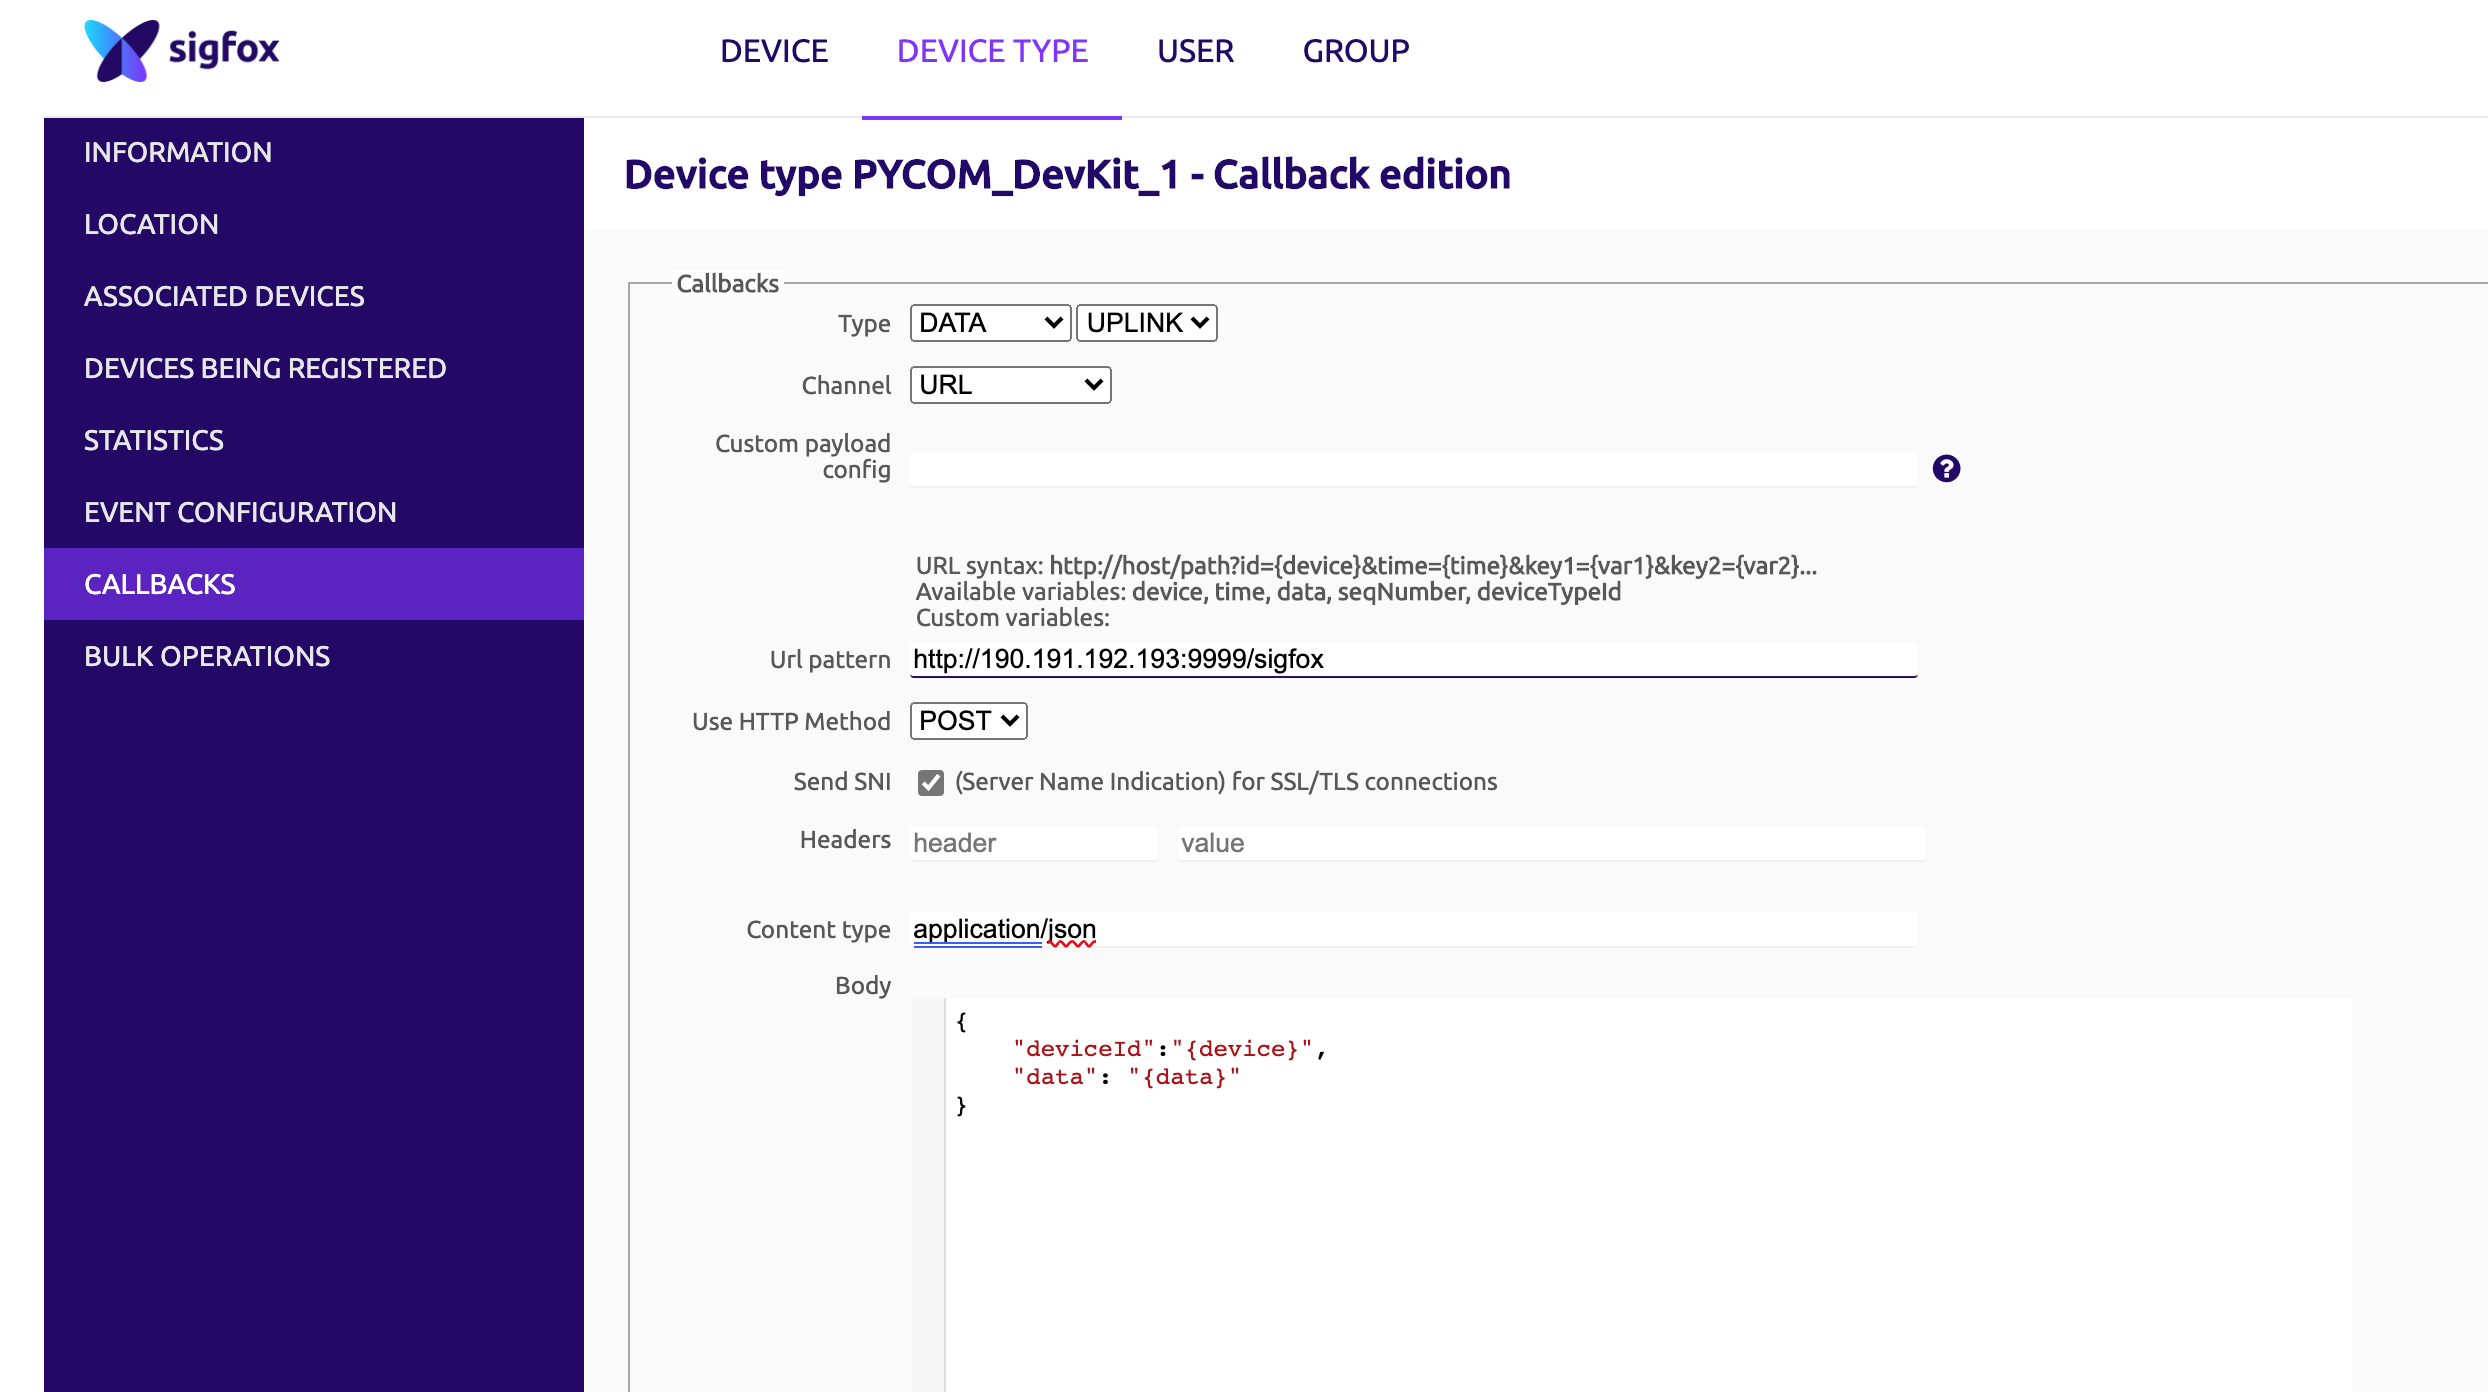
\includegraphics[width=1\columnwidth]{Pictures/sigfox-callback.png} }
\caption{Configuration d'un \textit{callback}.}
\label{fig-sigfox-callback}
\end{figure}

Ensuite, il faut déterminer l’adresse IP publique derrière votre \ac{NAT}\footnote{Un site comme \url{https://wtfismyip.com/} peut aider.}. L’URI de votre serveur sera quelque chose comme indiquée ci-dessous pour l'\textit{Url Pattern}, où \textit{aaa.bbb.ccc.ddd} représente l'adresse IP publique\footnote{Attention, certains opérateurs changent régulièrement l’adresse IP allouée au NAT. Il est donc préférable d’utiliser un DNS dynamique si vous voulez l’utiliser à long terme.}. 

\begin{termc}[backgroundcolor=\color{blue!10}, basicstyle=\ttfamily\small, escapechar=@]
http://@\textit{aaa.bbb.ccc.ddd}@:9999/sigfox
\end{termc}


     \vspace{1em}

Changez la méthode de \Index{GET} par un \Index{POST}, c’est quand même plus propre. Le GET étant un moyen de récupérer de l’information pas d’en transmettre si on veut rester compatible avec REST.

     \vspace{1em}

Ce n’est pas fini. Il faut maintenant formater le contenu. Dans Content type, remplacez la valeur par \texttt{application/json} car c’est ce que l’on sait faire de mieux. Dans la fenêtre en dessous, nous allons définir notre format JSON avec deux clés : \textit{deviceId} et \texttt{data}, suivies de deux variables entre accolades que Sigfox remplacera par les vraies valeurs.

     \vspace{1em}

Finalement, cliquez sur Ok. Maintenant, quand Sigfox recevra des données de l'objet, il enverra une requête POST à l'URI indiquée.

\subsubsection{Configuration du NAT}

Il vous reste à configurer le NAT de votre routeur d’accès pour que les paquets à destination du port 9999 (valeur choisie dans l’URI) TCP soient envoyés à l’adresse privée de votre ordinateur. La démarche est généralement la même : configurer DHCP pour que votre ordinateur ait toujours la même adresse dans la maison puis configurer le NAT pour que les paquets adressés à un port soit envoyé à cet ordinateur.\footnote{Si vous ne pouvez pas le faire, vous pouvez casser votre tirelire pour vous acheter un \ac{VPS} avec une adresse IP publique pour quelques par mois. Dans ce cas, il faudra installer Python3 et les modules nécessaires (Beebotte, cbor2...)}

\Index{Wireshark} peut vérifier que les requêtes traversent bien le NAT et arrive à votre ordinateur en regardant le trafic TCP sur le port 9999.

\subsubsection{Traitement des requêtes POST}

Les données contenues dans la requête POST venant du \textit{backend} de Sigfox seront transférer sur le lien \textit{\Index{loopback}} de l'ordinateur vers le port UDP 33033.
Le programme \pprog{display\_server.py}{plido-tp3} attendant les données sur ce port pourra être utiliser pour transformer la série temporelle codée en CBOR en structure JSON attendue par Beebotte. De cette manière, nous banalisons le programme qui pourra traiter ces trois sources d’information~:
\begin{itemize}
    \item objet émulé par un programme Python,
    \item LoPy avec Wi-Fi,
    \item LoPy avec Sigfox,
    \item et bientôt LoPy avec LoRaWAN.
\end{itemize}

     \vspace{1em}

 Le programme \pprog{generic\_relay.py}{plido-tp3} le fait pour Sigfox et différents serveurs LoRaWAN. Nous ne dévoilerons ici que les lignes liées au traitement de Sigfox.
 
 
 \pythonlst[firstline=54,lastline=68, firstnumber=54]{generic\_relay.py}
 
 On se rappelle du serveur \Index{Flask} que l'on avait vu au chapitre~\vref{chap-flask}, dans ce programme on retrouve les mêmes principes~:
 
 \begin{itemize}
     \item ligne 54, le decorateur permet de lier la fonction \texttt{get\_from\_sigfox} au chemin d'URI \texttt{/sigfox} pour la methode POST.
     \item ligne 57 désérialise le contenu du POST qui est contenu dans la variable \texttt{request}. Le paramètre \texttt{force} est là au cas où vous auriez oublié de mettre sur le \textit{backend} le format du contenu à \texttt{application/json}. Tout ce qu'il reçoit est considéré comme du JSON.
     \item lignes 62 à 64, si le POST contient des données (clé \texttt{data} dans l'objet JSON, alors elles sont envoyées sur le lien \textit{loopback} via la fonction \texttt{forward\_data}
     \item lignes 66 à 68, le POST est acquitté avec le status 200 pour indiquer que le traitement de la requête s'est bien déroulé.
 \end{itemize}
 
      \vspace{1em}

 A noter que la fonction \texttt{forward\_data} peut retourner une réponse qui sera envoyée au client HTTP. Pour Sigfox, cette possibilité n'est pas prise en compte car Sigfox n'autorise que 4 messages descendant par jour. Nous détaillerons son fonctionnement lorsque nous étudierons les réseaux LoRaWAN\footnote{Pour plus de détails sur l'envoi de messages descendant voir page~\pageref{chap—forward-data}.}.
 
 \pythonnxt[firstline=192,lastline=217, firstnumber=192]{generic\_relay.py}
 
 La partie principale du programme analyse les arguments utilisés lors de son appel. Si l'option \texttt{-v} est utilisé, le programme affichera les messages relayés. D'autres options sont définies pour modifier les numéro de port. Ces dernières sont utiles si ces programmes sont lancés sur un même machine dans le cloud.
 
 \subsubsection{Exemple}
 
L'exemple suivant trace le parcours d'une série temporelle depuis un LoPy jusuq'à son envoie au serveur Beebotte pour visualisation.

\begin{termc}[backgroundcolor=\color{gray!10}, basicstyle=\ttfamily\small, escapechar=@] 
>>> Running sigfox_temperature.py

>>>
>>>
[118]
[1895] 4
[1895, -4] 5
[1895, -4, -2] 6
[1895, -4, -2, 1] 7
[1895, -4, -2, 1, -3] 8
[1895, -4, -2, 1, -3, -1] 9
[1895, -4, -2, 1, -3, -1, 0] 10
[1895, -4, -2, 1, -3, -1, 0, 0] 11
[1895, -4, -2, 1, -3, -1, 0, 0, 6] 12
[1895, -4, -2, 1, -3, -1, 0, 0, 6, 2] 13
\end{termc}

Le LoPy collecte les mesures et construit sa série temporelle qui est envoyée quand la capacité de la trame est atteinte. Dans le cas de Sigfox, il s'agit de 12 octets, la dernière ligne montre que la capacité est dépassée, donc le dernier élément est retiré.

\begin{termc}[backgroundcolor=\color{palerod}, basicstyle=\ttfamily\small, escapechar=@] 
 >python3.5 generic_relay.py -v
SIGFOX POST RECEIVED
{'data': '@\ul{891907672321012220000006}@', 'deviceId': '4D3D0E'}
--UP-> b'891907672321012220000006'
no DW
<Response 0 bytes [200 OK]>
185.110.98.2 - - [24/Dec/2021 10:14:26] "POST /sigfox HTTP/1.1" 200 -
\end{termc}

Le programme \pprog{generic\_relay.py}{plido-tp3} reçoit la requête POST du réseau Sigfox sur le chemin d'URI \texttt{/Sigfox}. Elle contient l'élément CBOR envoyé par le LoPy. Ces données sont envoyée sur le port 33033. Aucune réponse n'est reçue, la requête POST est simplement acquittée.


\begin{termc}[backgroundcolor=\color{palerod}, basicstyle=\ttfamily\small, escapechar=@] 
 >python3 display_server.py
[{'data': 18.95, 'resource': 'temperature', 'ts': 1640337186000.0},
 {'data': 18.91, 'resource': 'temperature', 'ts': 1640337196000.0},
 {'data': 18.89, 'resource': 'temperature', 'ts': 1640337206000.0},
 {'data': 18.90, 'resource': 'temperature', 'ts': 1640337216000.0},
 {'data': 18.87, 'resource': 'temperature', 'ts': 1640337226000.0},
 {'data': 18.86, 'resource': 'temperature', 'ts': 1640337236000.0},
 {'data': 18.86, 'resource': 'temperature', 'ts': 1640337246000.0},
 {'data': 18.86, 'resource': 'temperature', 'ts': 1640337256000.0},
 {'data': 18.92, 'resource': 'temperature', 'ts': 1640337266000.0}]
\end{termc}

Le programme \pprog{display\_server.py}{plido-tp3} traite la donnée CBOR reçue sur le port 33033 et la convertie dans le format JSON attendu par Beebotte.

\section{Conclusion}

On a construit un prototype de capteur qui fonctionne sur Sigfox. À vous de l’améliorer. En particulier, il faut augmenter l’intervalle entre deux mesures qui a été fixé à 10 secondes pour ne pas avoir à faire des tests trop longs. Comme la taille d’un message est de 12 octets, CBOR va prendre 1 octet pour coder le tableau et la valeur de référence est codée sur 3 octets. Si les deltas sont petits, ils tiendront sur un octet. Il reste de la place pour 8 deltas. Donc, la période d’émission est de 90 secondes si les intervalles entre deux mesures restent à 10 secondes.

Comme Sigfox n'autorise que 140 messages par jours, la durée de mesure ne sera que de 210 minutes par jours, soit 3 heures et demie. Il est donc préférable de prendre des intervalles plus grands. Vous pouvez calibrer votre LoPy et votre programme de réception pour pouvoir suivre la température sur une journée. N'oubliez pas de changer également cette période dans le programme  \pprog{display\_server.py}{plido-tp3}.

      \vspace{1em}


Le programme \pprog{display\_server.py}{plido-tp3} permet de récolter des informations de plusieurs sources :
\begin{itemize}
    \item un programme en local qui émule les mesures,
    \item du réseau Wi-Fi,
    \item par l'intermédiaire de \pprog{generic\_relay.py}{plido-tp3} provenant d'un réseau LPWAN.
\end{itemize} 

      \vspace{1em}


Nous avons notre convention de représentation de l'information basée sur CBOR pour définir une série temporelle. En revanche, nous avions été obligés de modifier le programme  \pprog{display\_server.py}{plido-tp3} quand nous étions passé d'une série temporelle représentant l'évolution de l'humidité à une autre traitant de la température et si la période change.

      \vspace{1em}

Nous avons vu la différence entre les requêtes GET et POST qui induisent des comportements différents. Si GET est plus universel et peut fonctionner derrière un NAT, il demande des interrogation régulières pour savoir si la ressource à changée on non. POST impose que le serveur soit accessible et ainsi l'expose, mais les résultats sont reçus \"instantanément\". 

      \vspace{1em}
      
La notion de client et de serveur est floue, il ne peut pas être attribuée à un programme ou à un équipement, par exemple, le programme \pprog{display\_server.py}{plido-tp3} est serveur pour Sigfox et client pour Beebotte. Le site de Sigfox est serveur, si l'on utilise une méthode GET pour obtenir les données et client s'il fait un POST.
      
      \vspace{1em}

Pour revenir au paradigme de REST, nous avons, avec CBOR, défini le contenu de la ressource mais nous ne l'avons pas nommée. Le récepteur doit connaître le format (du CBOR contenant un série temporelle codée en différentiel) et ce qu'elle désigne.  C'est ce que nous allons voir dans la prochaine session avec le protocole \Index{CoAP} où nous pourrons définir, comme en HTTP, le nom de la ressource et son contenu.